\documentclass{article}
\usepackage{amsmath,accents}%
\usepackage{amsfonts}%
\usepackage{amssymb}%
\usepackage{comment}
\usepackage{graphicx}
\usepackage{mathrsfs}
\usepackage[utf8]{inputenc}
\usepackage{amsfonts}
\usepackage{amssymb}
\usepackage{graphicx}
\usepackage{mathrsfs}
\usepackage{setspace}  
\usepackage{amsthm}
\usepackage{nccmath}
\usepackage[UKenglish]{babel}
\usepackage{multirow}
\usepackage{enumerate}
\usepackage{listings}
\usepackage{pgf,tikz}
\usepackage{hyperref}
\usepackage{cleveref}
\usetikzlibrary{arrows}

\theoremstyle{plain}

\renewcommand{\baselinestretch}{1,4}
\setlength{\oddsidemargin}{0.5in}
\setlength{\evensidemargin}{0.5in}
\setlength{\textwidth}{5.4in}
\setlength{\topmargin}{-0.25in}
\setlength{\headheight}{0.5in}
\setlength{\headsep}{0.6in}
\setlength{\textheight}{8in}
\setlength{\footskip}{0.75in}

\newtheorem{theorem}{Teorema}[section]
\newtheorem{acknowledgement}{Acknowledgement}
\newtheorem{algorithm}{Algorithm}
\newtheorem{axiom}{Axiom}
\newtheorem{case}{Case}
\newtheorem{claim}{Claim}
\newtheorem{propi}[theorem]{Propiedades}
\newtheorem{condition}{Condition}
\newtheorem{conjecture}{Conjecture}
\newtheorem{coro}[theorem]{Corolario}
\newtheorem{criterion}{Criterion}
\newtheorem{defi}[theorem]{Definición}
\newtheorem{example}[theorem]{Ejemplo}

\theoremstyle{definition}
\newtheorem{exerciseaux}{Exercise}
\newtheorem{lemma}[theorem]{Lema}
\newtheorem{nota}[theorem]{Nota}
%\newtheorem{sol}{Solución}
%\newtheorem*{sol*}{Solution}
\newtheorem{prop}[theorem]{Proposición}
\newtheorem{remark}{Remark}
\newenvironment{exercise}[1]
  {\renewcommand\theexerciseaux{#1}\exerciseaux\label{ejer:#1}}
  {\endexerciseaux}
\newcounter{exercounter}[section]
\setcounter{exercounter}{\value{exerciseaux}}
\newenvironment{sol}{\begin{trivlist}
 \item[\hskip \labelsep {\textit{Solution}.}\hskip \labelsep]}{\end{trivlist}}

\newtheorem{dem}[theorem]{Demostración}

\newtheorem{summary}{Summary}

\providecommand{\abs}[1]{\lvert#1\rvert}
\providecommand{\norm}[1]{\lVert#1\rVert}
\providecommand{\ninf}[1]{\norm{#1}_\infty}
\providecommand{\numn}[1]{\norm{#1}_1}
\providecommand{\gabs}[1]{\left|{#1}\right|}
\newcommand{\bor}[1]{\mathcal{B}(#1)}
\newcommand{\parcial}[2]{\frac{\partial #1}{\partial #2}}
\newcommand{\secondparcial}[2]{\frac{\partial^2 #1}{\partial {#2}^2}}
\newcommand{\R}{\mathbb{R}}
\newcommand{\Q}{\mathbb{Q}}
\newcommand{\Z}{\mathbb{Z}}
\newcommand{\F}{\mathbb{F}}
\newcommand{\X}{\chi}
\providecommand{\Zn}[1]{\Z / \Z #1}
\newcommand{\resi}{\varepsilon_L}
\newcommand{\cee}{\mathbb{C}}
\providecommand{\conv}[1]{\overset{#1}{\longrightarrow}}
\providecommand{\gene}[1]{\langle{#1}\rangle}
\providecommand{\convcs}{\xrightarrow{CS}}
% xrightarrow{d}[d]
%\setcounter{exercise}{0}
\newcommand{\cicl}{\mathcal{C}}

\newenvironment{ejercicio}[2][Estado]{\begin{trivlist}
\item[\hskip \labelsep {\bfseries Ejercicio}\hskip \labelsep {\bfseries #2.}]}{\end{trivlist}}
%--------------------------------------------------------
\begin{document}

\title{Time Series Analysis - Exam }
\author{Javier Aguilar Martín}
\date{\today}
\maketitle

\section{Part I: R}

For this exercise I downloaded the data set and imported rows 61 to 208 (the columns with the quarterly rates) and named the two columns ``Quarter'' and ``Unemployment'' respectively. The data has not missing values so it is ready to be used. The dataframe is stored in a variable called \texttt{ts}. There is a total of $n=208$ rows.
\begin{exercise}{1}
\end{exercise}
\begin{sol}

The plot is in \Cref{Xt}. It has been created created using the following \texttt{R} script.
\begin{figure}
\centering
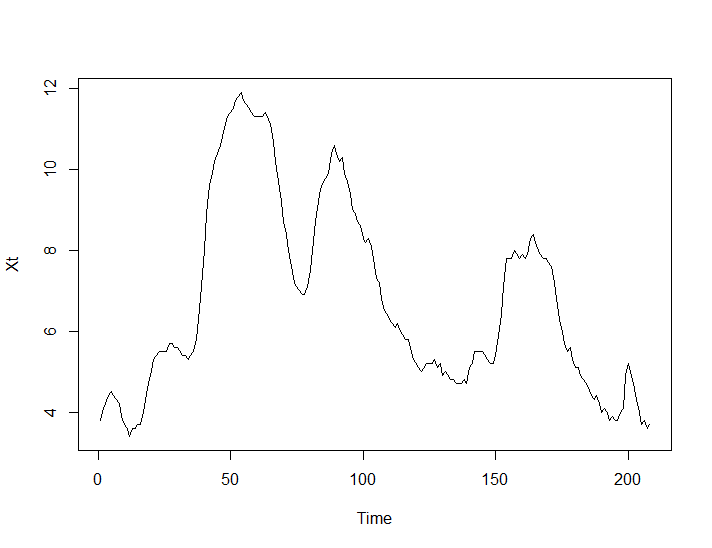
\includegraphics[scale=0.5]{Xt}
\caption{Plot of $X_t$.}\label{Xt}
\end{figure}


\lstset{language=R,
showstringspaces=false,
tab=\rightarrowfill}
\begin{lstlisting}
Xt <- ts$Unemployment
plot.ts(Xt)
\end{lstlisting}
\end{sol}

\begin{exercise}{2}
\end{exercise}
\begin{sol}
The plot is in \Cref{Yt}. It has been created created using the following \texttt{R} script.
\begin{figure}
\centering
\includegraphics[scale=0.5]{Yt}
\caption{Plot of $Y_t$.}\label{Yt}
\end{figure}

\lstset{language=R,
showstringspaces=false,
tab=\rightarrowfill}
\begin{lstlisting}
rates <- ts$Unemployment
yt <- diff(rates)
plot(yt, type = "l", xlab = "t", ylab = "Y_t")
\end{lstlisting}
\end{sol}


\begin{exercise}{3}
\end{exercise}
\begin{sol}
The plot of $X_t$ shows very recognizable trends of increasing and decreasing unemployment. Because of these trends, the series does not appear to be stationary. However, $Y_t$ does not seem to follow very clear patterns and it looks more stationary than the original one.
\end{sol}
\begin{exercise}{4}
\end{exercise}
\begin{sol}
The plot is in \Cref{acf}. It has been created created using the function \texttt{acf(Yt)} in \texttt{R}.
\begin{figure}
\centering
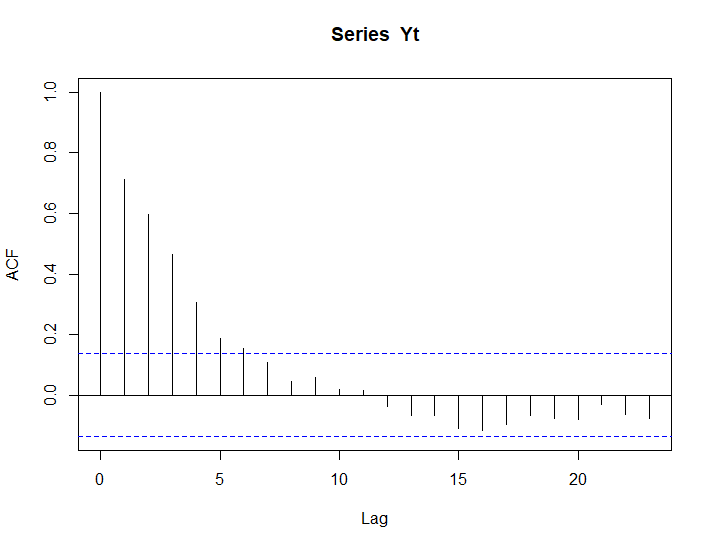
\includegraphics[scale=0.5]{acf}
\caption{Plot of the ACF estimates of $Y_t$.}\label{acf}
\end{figure}
\end{sol}
\begin{exercise}{5}
The plot is in \Cref{pacf}. It has been created created using the function \texttt{acf(Yt)} in \texttt{R}.
\begin{figure}
\centering
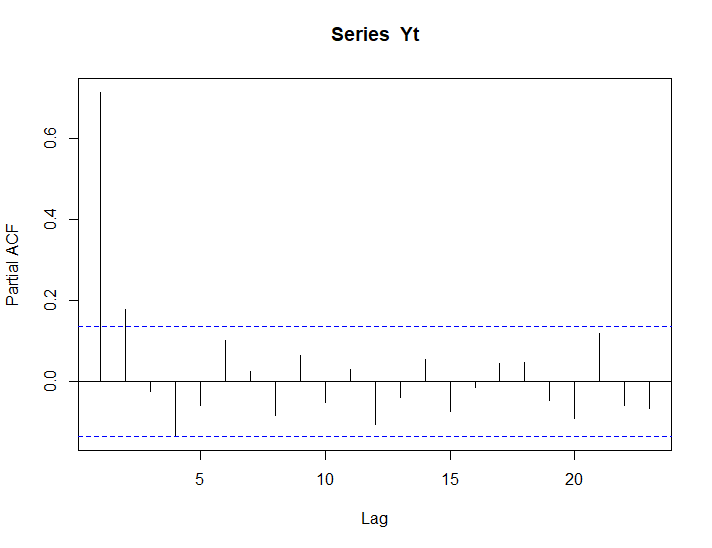
\includegraphics[scale=0.5]{pacf}
\caption{Plot of the PACF estimates of $Y_t$.}\label{pacf}
\end{figure}
\end{exercise}
\begin{sol}

\end{sol}
\begin{exercise}{6}
\end{exercise}
\begin{sol}
%https://www.kaggle.com/code/iamleonie/time-series-interpreting-acf-and-pacf
The ACF shows a geometrical decay and the PACF shows a significant lag at $p=1$. This suggest that $Y_t$ may be modelled using $AR(1)$. 
\end{sol}
\begin{exercise}{7}
\end{exercise}
\begin{sol}
As mentioned in the previous exercise, the PACF suggests using $AR(1)$. This means that the model is given by 
\[
Y_t = \epsilon_t +\phi Y_{t-1}
\]
where $\epsilon_t\sim WN(0,\sigma^2)$. 

The coeficients are estimated using \texttt{R} with three different methods as follows.
\lstset{language=R,
showstringspaces=false,
tab=\rightarrowfill}
\begin{lstlisting}
arima(Yt, order=c(1,0,0), method="CSS")

arima(Yt, order=c(1,0,0), method="ML")

arima(Yt, order=c(1,0,0), method="CSS-ML")
\end{lstlisting}

Using CSS the estimated value of $\phi$ is 0.7137 and the estimated value of $\sigma^2$ is 0.03472. There is also a small estimated intercept of -0.0041, suggesting that the series may not be perfectly centered at 0. ML and CSS-ML give both a common similar result to CSS, with a estimate for $\phi$ of 0.7147, an estimate for $\sigma^2$ of 0.03476 and an intercept of 0.0043.
\end{sol}
\begin{exercise}{8}
\end{exercise}
\begin{sol}
We estimate the $ARMA(p,q)$ model using \texttt{R} as follows.
\lstset{language=R,
showstringspaces=false,
tab=\rightarrowfill}
\begin{lstlisting}
library("forecast")
auto.arima(Yt, ic="bic")
\end{lstlisting}
The result is an $ARMA(2,0)$, or equivalently, an $AR(2)$ model with coefficients $\phi_1 = 0.59$, $\phi_2 = 0.173$ and $\sigma^2=0.03405$. 
\end{sol}
\begin{exercise}{9}
\end{exercise}
\begin{sol}
We run the following \texttt{R} lines to get a forecast for $Y_t$ according to the $AR(2)$ model.
\lstset{language=R,
showstringspaces=false,
tab=\rightarrowfill}
\begin{lstlisting}
fit <- Arima(Yt,c(2,0,0))
forecast(fit,2)
\end{lstlisting}
The predicted values are $Y_n=0.02563702$ and $Y_{n+1}= 0.03365256$. To obtain the unemployment rate we need to look at the value of $X_n$ and solve the differences. This value can be obtained using the function \texttt{tail(Xt,1)}, which returns 3.7. Then, we just have to compute
\[X_{n+1} = Y_n+X_n = 3.725637\]
and
\[
X_{n+2} = Y_{n+1} + X_{n+1} = 3.75929
\]
\end{sol}
\begin{exercise}{10}
\end{exercise}
\begin{sol}
One limitation is that ARMA asumes a constant variance. This is probably not true for the job market since it depends on policies and many other factors that may introduce more or less variability. Related to this, another limitation which mainly affects forecasting is that ARMA can't take into account external factors such as a financial crisis. 
\end{sol}

\section{Part II: Theory}

\begin{exercise}{1}
\end{exercise}
\begin{sol}
\begin{enumerate}[(a)]
\item 
I would first estimate the autocovariance coefficients $\gamma_0$, $\gamma_1$ and $\gamma_2$ using the sample autocovariance function
\[
\hat{\gamma}_h= \frac{1}{n}\sum_{t=1}^{n-h}(Y_t -\bar{Y})(Y_{t+h}-\bar{Y})
\]
for $h=0,1,2$. Then I would plug this values into the Yule-Walker equations to obtain estimates for $\phi_1$ and $\phi_2$ as follows.
\[
\begin{pmatrix}
\hat{\phi}_1\\
\hat{\phi}_2
\end{pmatrix}=\begin{pmatrix}
\hat{\gamma}_0 & \hat{\gamma}_1\\
\hat{\gamma}_1 & \hat{\gamma}_0
\end{pmatrix}^{-1}\begin{pmatrix}
\hat{\gamma}_1\\
\hat{\gamma}_2
\end{pmatrix}
\]
More explicitly this gives
\begin{align*}
\hat{\phi}_1 & =\frac{\hat{\gamma}_1(\hat{\gamma}_0-\hat{\gamma}_2)}{\hat{\gamma}_0^2-\hat{\gamma}_1^2}\\
\hat{\phi}_1 & = \frac{\hat{\gamma}_1(\hat{\gamma}_2-\hat{\gamma}_0)}{\hat{\gamma}_0^2-\hat{\gamma}_1^2}=-\hat{\phi}_1
\end{align*}
Finally, $\sigma^2$ can be estimated from the Yule-Walker equations using the previous estimates as 
\begin{align*}
\hat{\sigma}^2 &= \hat{\gamma}_0 -\hat{\phi}_1\hat{\gamma}_1 - \hat{\phi}_2\hat{\gamma}_2\\
 & =  \hat{\gamma}_0 +\hat{\phi}_1(\hat{\gamma}_2 - \hat{\gamma}_1)\\
 & = \hat{\gamma}_0 +\frac{(\hat{\gamma}_2 - \hat{\gamma}_1)\hat{\gamma}_1(\hat{\gamma}_0-\hat{\gamma}_2)}{\hat{\gamma}_0^2-\hat{\gamma}_1^2}
\end{align*}

\item Let $\phi = (\phi_1,\phi_2)^T$ and similarly $\tilde{\phi}$. Let $\Gamma = (\gamma_{i-j})_{i,j=1}^2$ and similarly $\tilde{\Gamma}$. We know that asymptotically $\phi$ follows a normal distribution of mean $\tilde{\phi}$ and variance $\frac{\sigma^2}{n}\Gamma^{-1}$. Since $\tilde{\sigma}^2\xrightarrow{p}\sigma^2$ as $n\to\infty$, we may replace $\sigma^2$ by $\tilde{\sigma}^2$ and similarly $\Gamma$ by $\tilde{\Gamma}$ in order to do calculations. 

%https://stats.stackexchange.com/questions/22879/linear-combination-of-two-dependent-multivariate-normal-random-variables
We can obtain the quantity $\phi_1-2\phi_2$ can be obtained as a result of the product $(1,-2)\phi$, and therefore asyntotically follows a normal distribution with mean $\mu = \hat{\phi}_1-2\hat{\phi}_2$ and variance estimated by 
\[
\tau^2= \frac{\tilde{\sigma}^2}{n}(1,-2)\tilde{\Gamma}^{-1}(1,-2)^T= \frac{\tilde{\sigma}^2}{n}\frac{\tilde{\gamma_0}}{\hat{\gamma}_0^2-\hat{\gamma}_1^2}
\]
Therefore, a 95\% interval for $\phi_1-2\phi_2$ has bounds
\[
\mu \pm z_{0.025}\frac{\tau}{\sqrt{n}}.
\]

A test for the equality $\phi_1 = 2\phi_2$ would consist of checking whether 0 is the the above confidence interval or not.
\end{enumerate}
\end{sol}

\begin{exercise}{2}
\end{exercise}
\begin{sol}
\begin{enumerate}[(a)]
\item
\begin{enumerate}[(i)]
\item We compute first $E(Y_t)$ using the law of iterated expectations.
\[
E(Y_t)=E(\sigma_t\epsilon_t)= E(E(\sigma_t\epsilon_t\mid \mathcal{F}_{t-1}))=E(\sigma_tE(\epsilon_t\mid \mathcal{F}_{t-1}))=E(\sigma_tE(\epsilon_t))=0.
\]
Now we compute $E(Y_t)$ using the mean of the folded normal distribution.
\begin{align*}
E(|Y_t|)&= E(|\sigma_t\epsilon_t|)\\
& = E(\sigma_t|\epsilon_t|)\\
&=E((b_0+b_1|Y_{t-1}|+b_2|Y_{t-2}|)|\epsilon_t|)\\
&=(b_0+b_1E(|Y_{t-1}|)+b_2E(|Y_{t-2}|))E(|\epsilon_t|)\\
&=(b_0+b_1E(|Y_t|)+b_2E(|Y_{t}|))\sqrt{\frac{2}{\pi}}
\end{align*}
From this we deduce that
\[
E(|Y_t|)=\frac{b_0\sqrt{\frac{2}{\pi}}}{1-\sqrt{\frac{2}{\pi}}(b_1+b_2)}
\]
\item Since $E(Y_t)=0$ we have for $h>0$
\begin{align*}
\gamma_h & = \mathrm{cov}(Y_t, Y_{t-h})=E(Y_tY_{t+h})=E(E(Y_tY_{t-h}\mid \mathcal{F}_{t-1}))=E(Y_{t-h}E(Y_t\mid\mathcal{F}_{t-1}))\\
& = E(Y_{t-h}E(\sigma_t\epsilon_t))=0
\end{align*}
So the ACF is 0 for $h>0$. For the PACF consider
\[
Y_{h+1}- E(Y_{h+1}\mid Y_h,\dots, Y_2)=Y_{h+1}-E(\sigma_{h+1}\epsilon_{h+1}\mid Y_h,\dots, Y_2)=Y_{h+1}
\]
So $\phi_{hh}=\mathrm{corr}(Y_{h+1},Y_1-E(Y_1\mid X_h,\dots, Y_2))=0$ since $Y_{h+1}$ and $Y_1$ are uncorrelated.
\end{enumerate}
\item We can rewrite $Y_t$ as an $AR(2)$ process in $|Y_t|$ with a not i.i.d normal white noise as follows.
\begin{align*}
|Y_t| & = \sigma_t + |Y_t|-\sigma_t\\
& = b_0+b_1|Y_{t-1}| + b_2|Y_{t-1}| + \sigma_t(|\epsilon_t|-1)\\
& = b_0+b_1|Y_{t-1}| + b_2|Y_{t-1}|+v_t
\end{align*}
This allows for least square estimation by considering the system
\[Y=Xb+V\]
where $Y=(|Y_1|,\dots, |Y_n|)^T$, $b = (b_0,b_1,b_2)^T$, $V=(v_1,\dots, v_n)^T$ and
\[
X = \begin{pmatrix}
1 & |Y_0| & |Y_1|\\
1 & |Y_1| & |Y_2|\\
 & \cdots & \\
1 & |Y_{n-1}| & |Y_n| 
\end{pmatrix}
\]
\end{enumerate}
We can set $Y_0 = E(Y_t)=0$. Therefore, a LSE for $b$ is given by 
\[\tilde{b} = \mathrm{argmin}_{\theta\in\R^3}||Y-X\theta|| = (X^TX)^{-1}X^T Y.\]

Another possibility is maximum likelihood estimation. Notice that $Y_t\mid \mathcal{F}_{t-1}\sim N(0,\sigma_t^2)$ where $\sigma_t^2 = b_0+b_1|Y_{t-1}|+b_2|Y_{t-2}|$. Therefore, the conditional probability density can be written as
\[f(Y_t\mid \mathcal{F}_{t-1})=f(Y_t\mid Y_{t-1}, Y_{t-2})=(2\pi\sigma_t)^{\frac{-1}{2}}\exp\left(-\frac{Y_t^2}{\sigma_t^2}\right).\]
Iterating this conditional argument we obtain
\begin{align*}
f(Y_n,\dots, Y_1\mid Y_0) &=f(Y_n\mid Y_{n-1})f(Y_{n-1}\mid Y_{n-2})\cdots f(Y_1\mid Y_0)\\
\log{f(Y_n,\dots, Y_1\mid Y_0)}  & =\sum_{t=1}^n \log f(Y_t\mid Y_{t-1})\\
& = -\frac{1}{2}\left(n\log{2\pi} +\sum_{t=1}^n\sigma_t^2+\sum_{t=1}^n\frac{Y_t^2}{\sigma_t^2}\right).
\end{align*}
Again, we may set $Y_0=0$ and the above function can be optimised numerically.
\end{sol}
\end{document}